\section{Problem Formulation} \label{sec:problem_formulation}
Fig. \ref{fig:controller-setup} shows a simplified top-level architecture of the control problem. Here, the controller is in charge of managing the energy of the energy storage and utility-owned generator of a distribution feeder. This is an example feeder comprised of five buses, two PVs (Pv1, PV2), four loads (D2, D3, D4 \& D5), four lines (L1, L2, L3 \& L4),  two energy storage (ES1, ES2), and one utility-owned generator (G). The energy management system  (EMS) shown in  Fig. \ref{fig:controller-setup} is taking the system status, forecasts, and RTP data as input and determining the power output of the controllable DERs, which in this case are the two energy storage and the utility-owned generator.

\begin{figure}
\centering
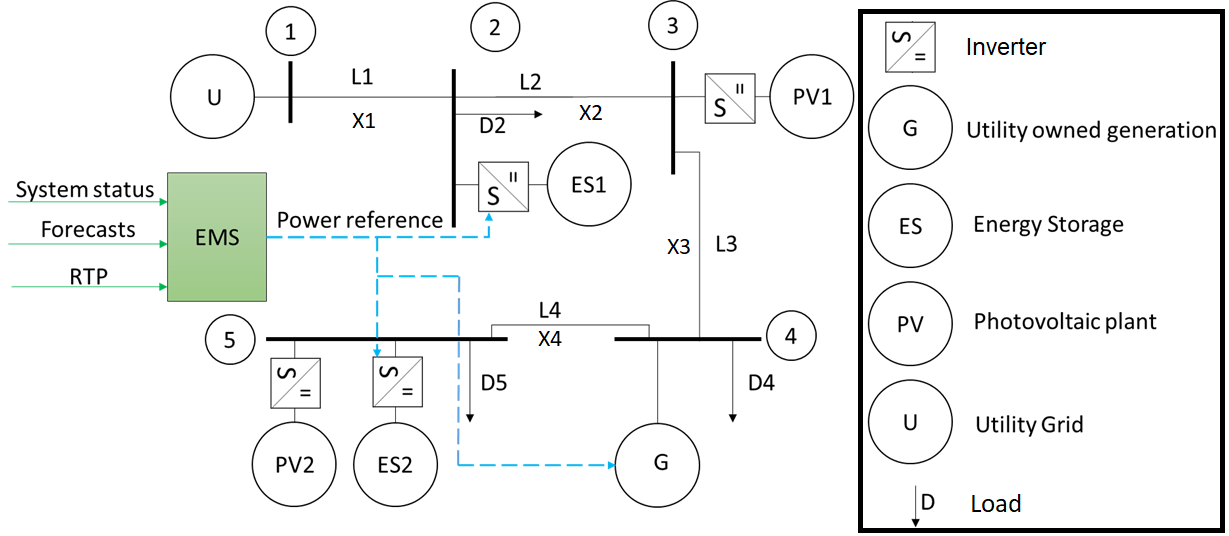
\includegraphics[width = \linewidth]{figs/A82/controller_setup2.png}
\caption{Simplified top-level controller architecture}
\label{fig:controller-setup}
\end{figure}

To incorporate the future forecasts and RTP as well as the current system status a graph is constructed from both the present and future status of the system. Fig. \ref{fig:F1_1_Dis} represents a simple example graph which is constructed assuming relevant forecasts and RTP is available for the system to generate states 15, 30 and 45 minutes in the future. . The values on top of the figure represent time. T = 0 represents the present and T = 15, 30 and 45 represents future states 15, 30 and 45 minutes in the future. The boxes with numbers inside are the nodes of the graph. The numbers represent the percentage of total energy storage (ES) capacity available to the system. The arrows represent the edges of the graph. In this case the edges are unidirectional. This is because it is impossible to return to a past node from a future node. The edges represents the cost of going from one node to the another. The graph is constructed considering an operation between 20\% to 80\% of total ES capacity and discretization steps of 20\%. It is also considered that the system has the capacity to discharge 40\% of the total energy capacity at most and charge up to 20\% of the total energy capacity at most within 15 minutes. Taking all these things into consideration the graph in fig. \ref{fig:F1_1_Dis} is generated and the problem that needs to be solved is to find the most cost optimum path to go from the starting node at T = 0 to any node at T = 45 while maintaining system constraints.

% The cost optimum solution is found by finding the optimum path in a graph search problem formulated to reflect different operation scenarios of the system. Fig. \ref{fig:F1_1_Dis} represents a simple example of the graph search formulation of the problem. The values on top of the figure represent the current time-step. The values inside the boxes represent the percentage of total energy storage (ES) capacity available in the system. These boxes are the nodes of the graph. The arrows from one box to the next represent the edges of the graph. It is assumed that the system power demand is constant between time steps. The system status at T=0 is known from the current measurement. The nodes at T=15, T=30, and T=45 are created based on forecasted values. The target of the solution is to find the most cost-optimum path to reach T=45 based on the predictions available. 

\begin{figure}[!h]
\centering
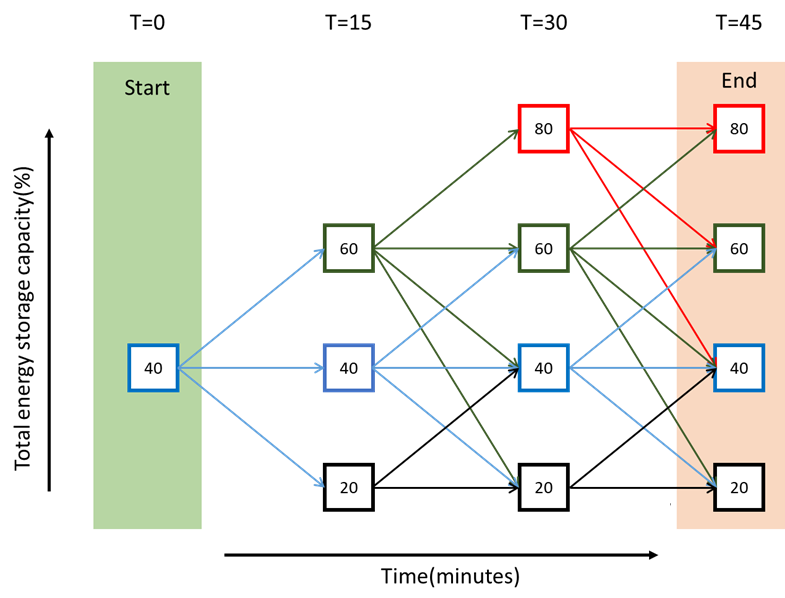
\includegraphics[width = .8\linewidth]{figs/A82/A8_graph_22.png}
\caption{Graph formulation}
\label{fig:F1_1_Dis}
\end{figure}